\documentclass[handout,noauthor,nooutcomes]{ximera}

\input{../../../preamble.tex}

\title[Collaborate:]{Considering surfaces}

\begin{document}
\begin{abstract}
We think about surfaces in different ways. 
\end{abstract}
\maketitle

\textbf{Work in groups of 3--4, writing your answers on a separate
  sheet of paper.}


\section{Considering tables}


Let $F:\R^2\to\R$ be a differentiable function that is roughly
described by the following table of values:
\begin{image}
  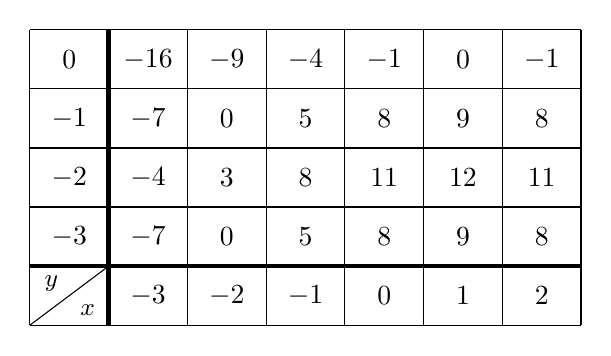
\begin{tikzpicture}[x=1cm,y=.75cm]
    \draw (0,0) grid [step=1] (7,5);
    
    \draw[ultra thick] (0,1)--(7,1);
    \draw[ultra thick] (1,0)--(1,5);
    
    \draw (0,0) -- (1,1);
    \node at (.4,.9) [below left,inner sep=1pt] {\small$y$};
    \node at (0.6,.1) [above right,inner sep=1pt] {\small$x$};
    
    %% y-values
    \node at (0.5,4.5) {$0$};
    \node at (0.5,3.5) {$-1$};
    \node at (0.5,2.5) {$-2$};
    \node at (0.5,1.5) {$-3$};

    
    %% z-values
    %% top
    \node at (1.5,4.5) {$-16$};
    \node at (2.5,4.5) {$-9$};
    \node at (3.5,4.5) {$-4$};
    \node at (4.5,4.5) {$-1$};
    \node at (5.5,4.5) {$0$};
    \node at (6.5,4.5) {$-1$};
    
    %% 
    \node at (1.5,3.5) {$-7$};
    \node at (2.5,3.5) {$0$};
    \node at (3.5,3.5) {$5$};
    \node at (4.5,3.5) {$8$};
    \node at (5.5,3.5) {$9$};
    \node at (6.5,3.5) {$8$};
    
    %% 
    \node at (1.5,2.5) {$-4$};
    \node at (2.5,2.5) {$3$};
    \node at (3.5,2.5) {$8$};
    \node at (4.5,2.5) {$11$};
    \node at (5.5,2.5) {$12$};
    \node at (6.5,2.5) {$11$};
    
    %% 
    \node at (1.5,1.5) {$-7$};
    \node at (2.5,1.5) {$0$};
    \node at (3.5,1.5) {$5$};
    \node at (4.5,1.5) {$8$};
    \node at (5.5,1.5) {$9$};
    \node at (6.5,1.5) {$8$};
    
    %% bottom row
    \node at (1.5,.5) {$-3$};
    \node at (2.5,.5) {$-2$};
    \node at (3.5,.5) {$-1$};
    \node at (4.5,.5) {$0$};
    \node at (5.5,.5) {$1$};
    \node at (6.5,.5) {$2$};
  \end{tikzpicture}
\end{image}

\begin{problem}
  Write the value of $F(-2,-1)$.
\end{problem}


\begin{problem}
  Estimate $F^{(1,0)}(-2,-1)$.
\end{problem}

\begin{problem}
  Estimate $F^{(0,1)}(-2,-1)$.
\end{problem}

\begin{problem}
  Estimate $\grad F(-2,-1)$.
\end{problem}

\begin{problem}
  If you were to leave the point $(-2,-1)$ in the direction of the
  gradient, what value would you find? \textbf{Explain why this makes
    sense.}
\end{problem}


\begin{problem}
  Use your computations above to estimate the formula for a plane
  tangent to $F(x,y)$ at the point $(-2,-1)$.
\end{problem}

\begin{problem}
  Sketch the level curve $F(x,y) = 1$ on the grid above.
\end{problem}

\section{Considering level sets}


Consider the following contour plot for $z=G(x,y)$:
\begin{image}[5in]
  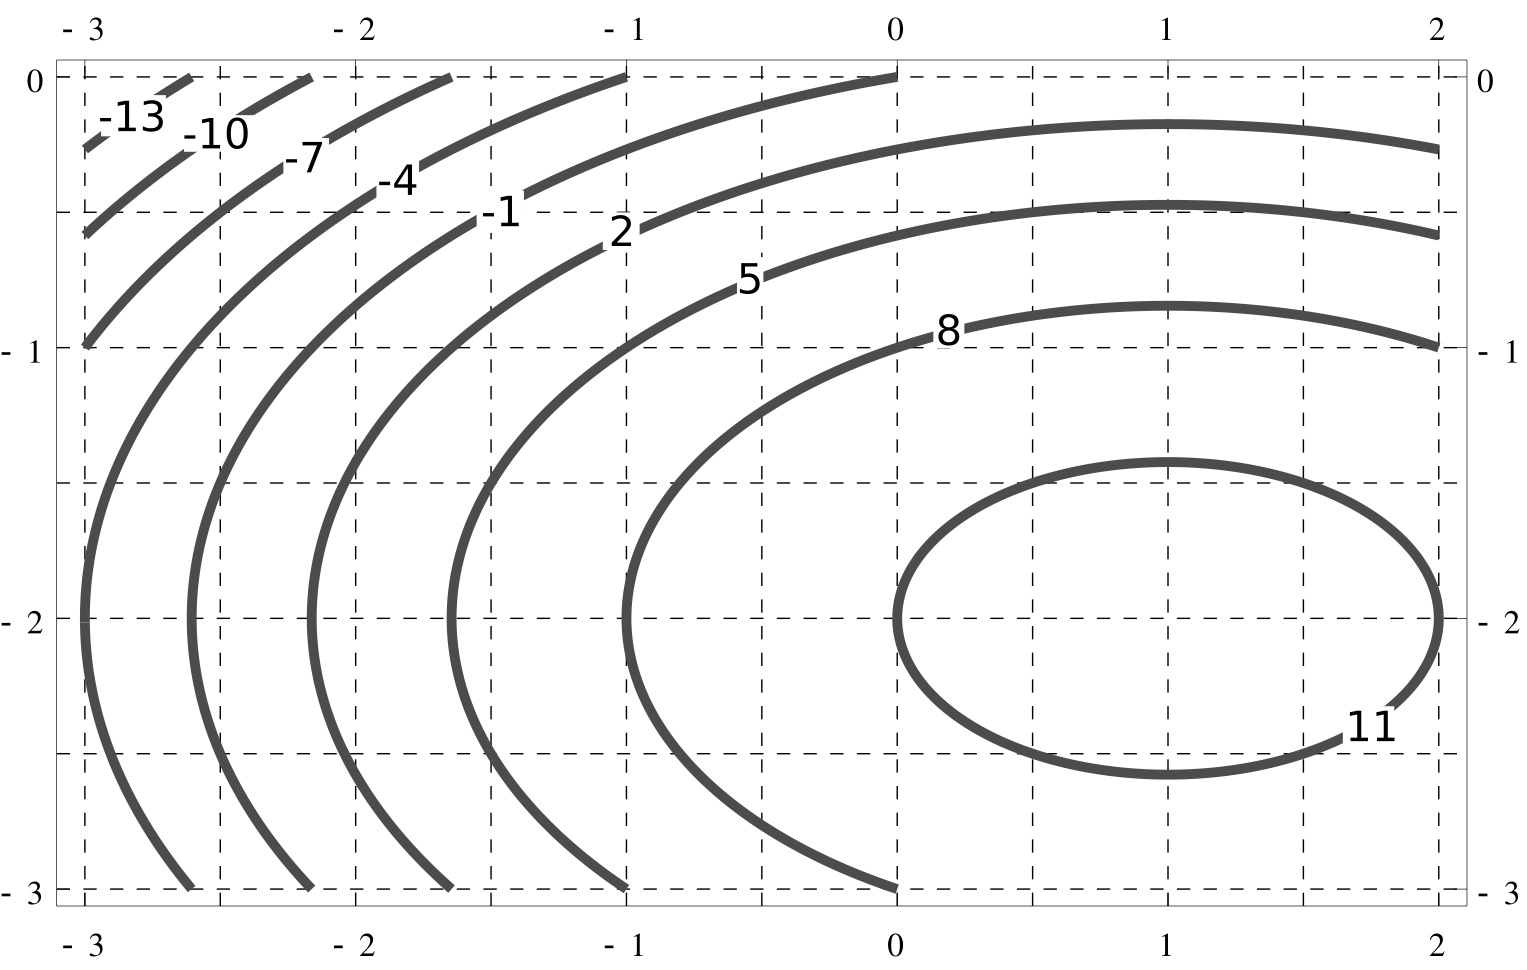
\includegraphics{contours.png}
\end{image}

\begin{problem}
  What does a contour plot like this represent? Circle one:
 % \begin{multicols}{2}
    \begin{itemize}
    \item A subset of $\R^2$
    \item A subset of $\R^3$
    \end{itemize}
  %\end{multicols}
\end{problem}

\begin{problem}
  Estimate the value of $G(0,-1)$.
\end{problem}

\begin{problem}
  Estimate $G^{(1,0)}(0,-1)$.
\end{problem}

\begin{problem}
  Estimate $G^{(0,1)}(0,-1)$.
\end{problem}

\begin{problem}
  Estimate $\grad G(0,-1)$.
\end{problem}

\begin{problem}
  If you were to leave the point $(0,-1)$ in the direction of the
  gradient, what value would you find? \textbf{Explain why this makes
    sense.}
\end{problem}

\begin{problem}
  Use your computations above to estimate the formula for a plane
  tangent to $G(x,y)$ at the point $(0,-1)$.
\end{problem}

\section{Considering algebra}

Let  $H:\R^2\to\R$ be described by:
\[
H(x,y) = -1 + 2 x - x^2 - 12 y - 3 y^2
\]
As a gesture of friendship, we have included a graph $z = H(x,y)$:
\begin{image}
  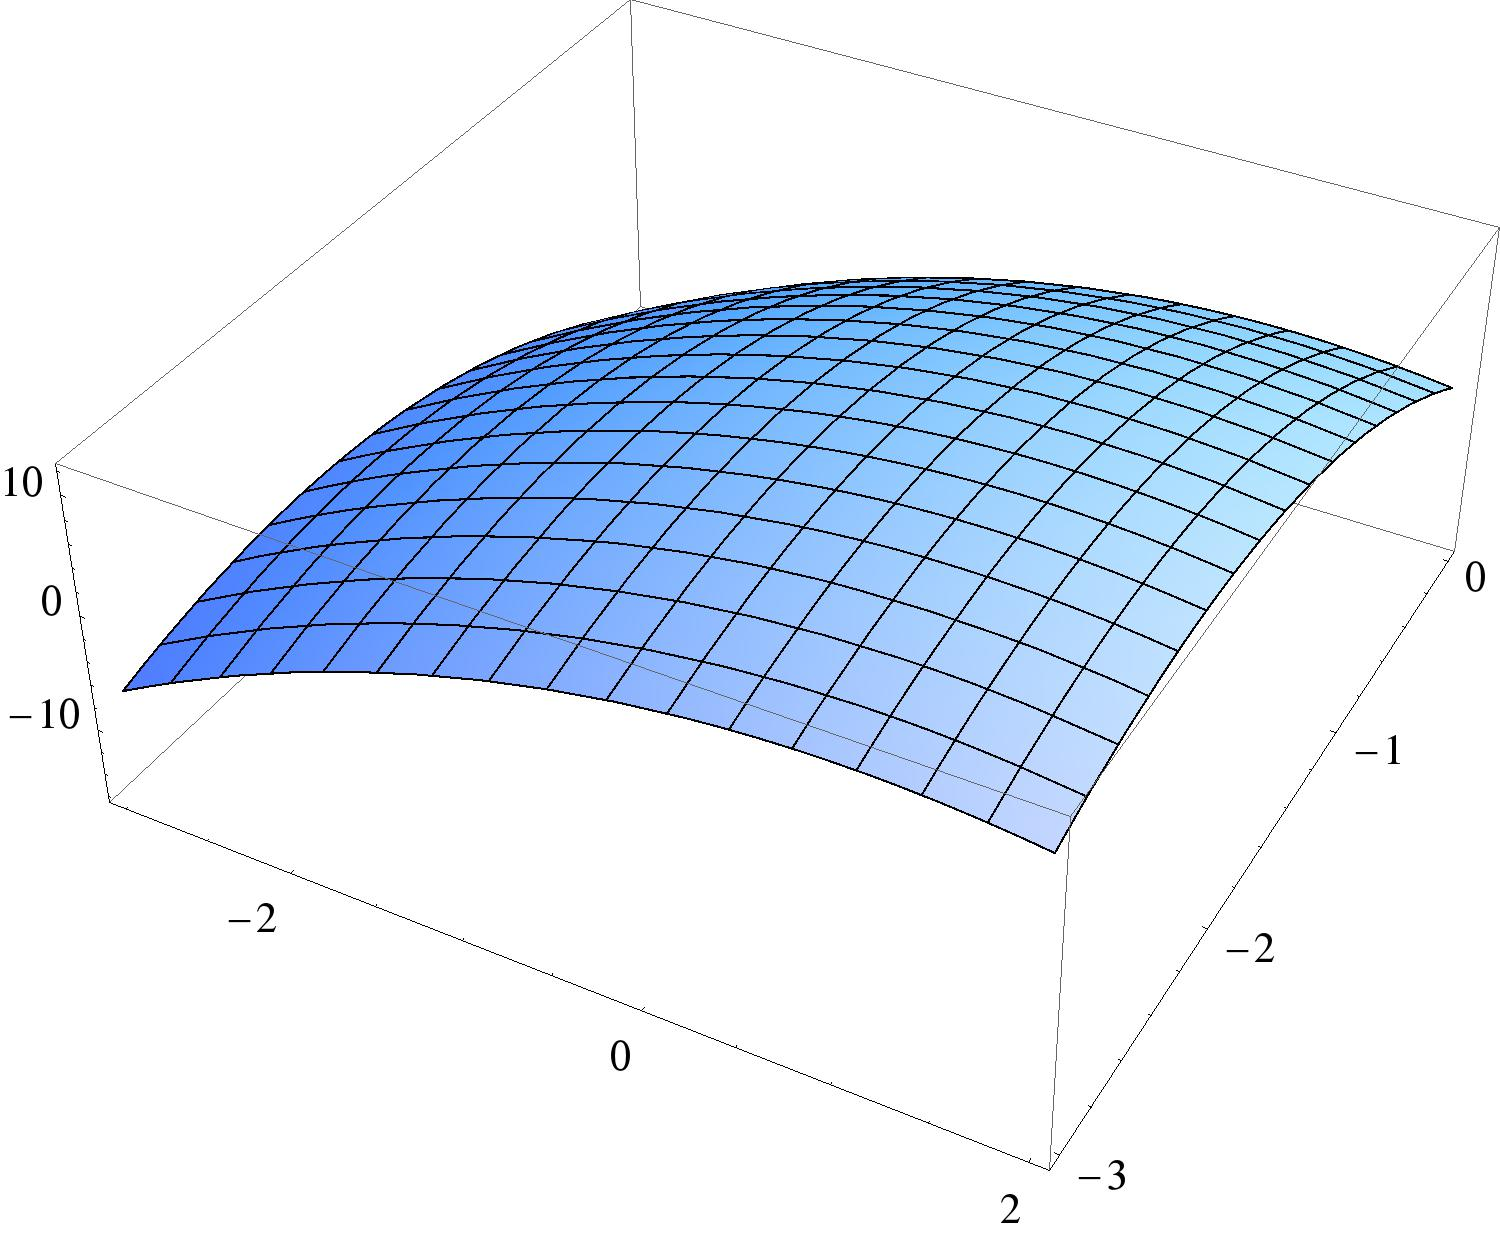
\includegraphics{surfacePlot.jpg}
\end{image}

\begin{problem}
  Compute:
    \begin{enumerate}
    \item $H(-2,-1)$
    \item $H(0,-1)$
    \end{enumerate}
\end{problem}

\begin{problem}
  Compute:
    \begin{enumerate}
    \item $H^{(1,0)}(-2,-1)$
    \item $H^{(0,1)}(-2,-1)$
    \item $H^{(1,0)}(0,-1)$
    \item $H^{(0,1)}(0,-1)$
    \end{enumerate}
\end{problem}

\begin{problem}
  Compare and contrast the functions $F$, $G$, and $H$. Discuss.
\end{problem}





\end{document}
